\chapter{Propostas Tecnológicas}

A análise de dados é uma disciplina essencial que desempenha um papel fundamental na tomada de decisões estratégicas e no impulsionamento dos negócios. Com o avanço da era do Big Data, onde uma quantidade massiva de informações é gerada e coletada diariamente, as empresas têm reconhecido cada vez mais a importância de investir em tecnologias e práticas analíticas para extrair insights acionáveis a partir desses dados. Esses insights podem fornecer uma visão abrangente do mercado, identificar oportunidades de crescimento, otimizar operações e melhorar o atendimento ao cliente, conferindo uma vantagem competitiva significativa às organizações que são capazes de aproveitar ao máximo a análise de dados em suas estratégias de negócio \cite{mayer2013big, chen2012business, reddy2013data, watson2010current, white2012hadoop}.

Com essas informações organizadas e disponíveis, tais empresas podem direcionar seus serviços de maneira mais eficaz, desenvolvendo estratégias baseadas em dados concretos e atualizados, contribuindo para o sucesso de seus negócios \cite{chen2012business}.
Entretanto, para transformar esses dados brutos em informações úteis, é necessária uma série de operações, muitas vezes resumidas no processo de Extração, Transformação e Carga (ETL). Este processo envolve a coleta de dados de várias fontes, a transformação desses dados para um formato adequado para análise, e, finalmente, a ingestão dos dados transformados em um sistema de destino para fácil acesso e análise \cite{vassiliadis2002conceptual}.

A adoção de um banco de dados é fundamental para a efetiva implementação do processo de ETL e análise de dados em empresas. Um banco de dados confiável e eficiente desempenha um papel crucial na organização e armazenamento dos dados coletados, permitindo que sejam facilmente acessados e utilizados para análise \cite{elmasri2019fundamentals}. Um banco de dados relacional é uma opção comumente adotada pelas organizações, pois oferece a capacidade de estruturar e relacionar os dados de forma coesa, tornando-os mais compreensíveis e significativos para os usuários \cite{date2003introduction}. Com a utilização de um banco de dados relacional, as empresas podem realizar consultas complexas e obter insights valiosos por meio de operações de junção e agregação dos dados \cite{connolly2014database}. Além disso, a integridade dos dados é assegurada por meio de restrições e relacionamentos definidos no banco de dados, garantindo a consistência dos dados ao longo do tempo \cite{silberschatz2019database}.


A empresa em questão é uma provedora de internet, que atua no mercado B2B (Business to Business), ou seja, atende outras empresas. A empresa possui cerca de 100 funcionários, e está localizada na cidade de São Paulo. Atualmente a empresa utiliza as informações do site da Receita Federal para obter os dados cadastrais dos CNPJs que são abertos no Brasil. Essa informação é utilizada para que o time de prospecção do cliente possa realizar o primeiro contato para oferecer os serviços da empresa. Atualmente, os dados dessa empresa são disponibilizados em um servidor on-premisse, onde um time realiza a extração dos dados do site da receita federal e disponibiliza em um arquivo excel, que é compartilhado com os times de prospecção do cliente e análise de dados através desse servidor. Boa parte desse processo exige a atuação humana, o que torna o processo lento e suscetível a erros. 

As construções dos paineis do time de análise também se baseiam nesses arquivos Excels e quando ocorre a atualização erronea desse arquivo, os painéis tendem a apresentar informações incorretas, ou até mesmo apresentar erro na própria ferramenta. Além disso, a informação não é estruturada da maneira correta, o que dificulta a análise dos dados e a tomada de decisão. Por fim, a informação não é atualizada com tempo hábil para prospecção do cliente, dando uma desvantagem competitiva para a empresa.

Este projeto tem como objetivo construir uma solução que seja em sua maior parte automatizada, realizando os processos atuais de forma 
mais eficiente e com menos intervenção humana. É do interesse também da empresa preservar os custos atuais, ou até mesmo reduzi-los. Considerando esse requisito e o objetivo do projeto, a solução proposta é a adoção de uma solução em nuvem, que permita a escalabilidade e o processamento eficiente dos dados. A solução proposta também envolve a passagem de conhecimento, bem como workshops com os times interessados para a apresentação e treinamento da solução proposta.

\section{Proposta 1}

\begin{figure}[H]
    \centering
    \caption{Arquitetura proposta 1}
    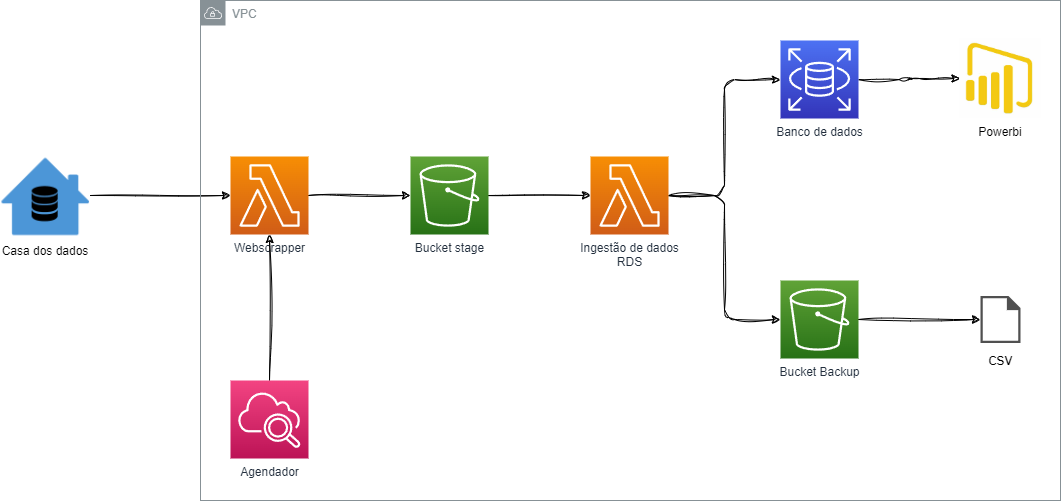
\includegraphics[scale = 0.7]{imagens/arquitetura_aws.png}
    
    \caption*{Arquitetura de solução proposta 1.}
    \end{figure}

Considerando o objetivo do projeto e o levantamento de requisitos feito junto aos responsáveis, foi possível construir a proposta de uma arquitetura de solução utilizando a provedora de serviços em nuvem AWS. Primeiramente, foi construído o modelo visual da solução em alto nível, visando a melhor visualização do que seria necessário para a construção da solução em termos de ferramentas. A partir desse primeiro modelo apresentado na figura \ref{fig:imagens/arquitetura_aws.png}, foi possível realizar uma análise mais detalhada dos serviços necessários para a construção da solução.



\begin{enumerate}
    \item Elmasri, R., & Navathe, S. B. (2019). Fundamentals of database systems. Pearson.
    \item Date, C. J. (2003). An introduction to database systems. Addison-Wesley.
    \item Connolly, T. M., & Begg, C. E. (2014). Database systems: A practical approach to design, implementation, and management. Pearson.
    \item Silberschatz, A., Korth, H. F., & Sudarshan, S. (2019). Database system concepts. McGraw-Hill Education.
    \item Reddy, C. K. (2013). Data analytics: From Big Data to big impact. International Journal of Information Management, 33(5), 761-764.
    \item Golfarelli, M., Rizzi, S., & Cella, I. (2003). Beyond data warehousing: What's next in business intelligence? In Proceedings of the 7th ACM international workshop on Data warehousing and OLAP (pp. 1-8).
    \item Ramakrishnan, R., & Gehrke, J. (2003). Database management systems. McGraw-Hill Education.
    \end{enumerate}